


\tikzset{every picture/.style={line width=0.75pt}} %set default line width to 0.75pt        

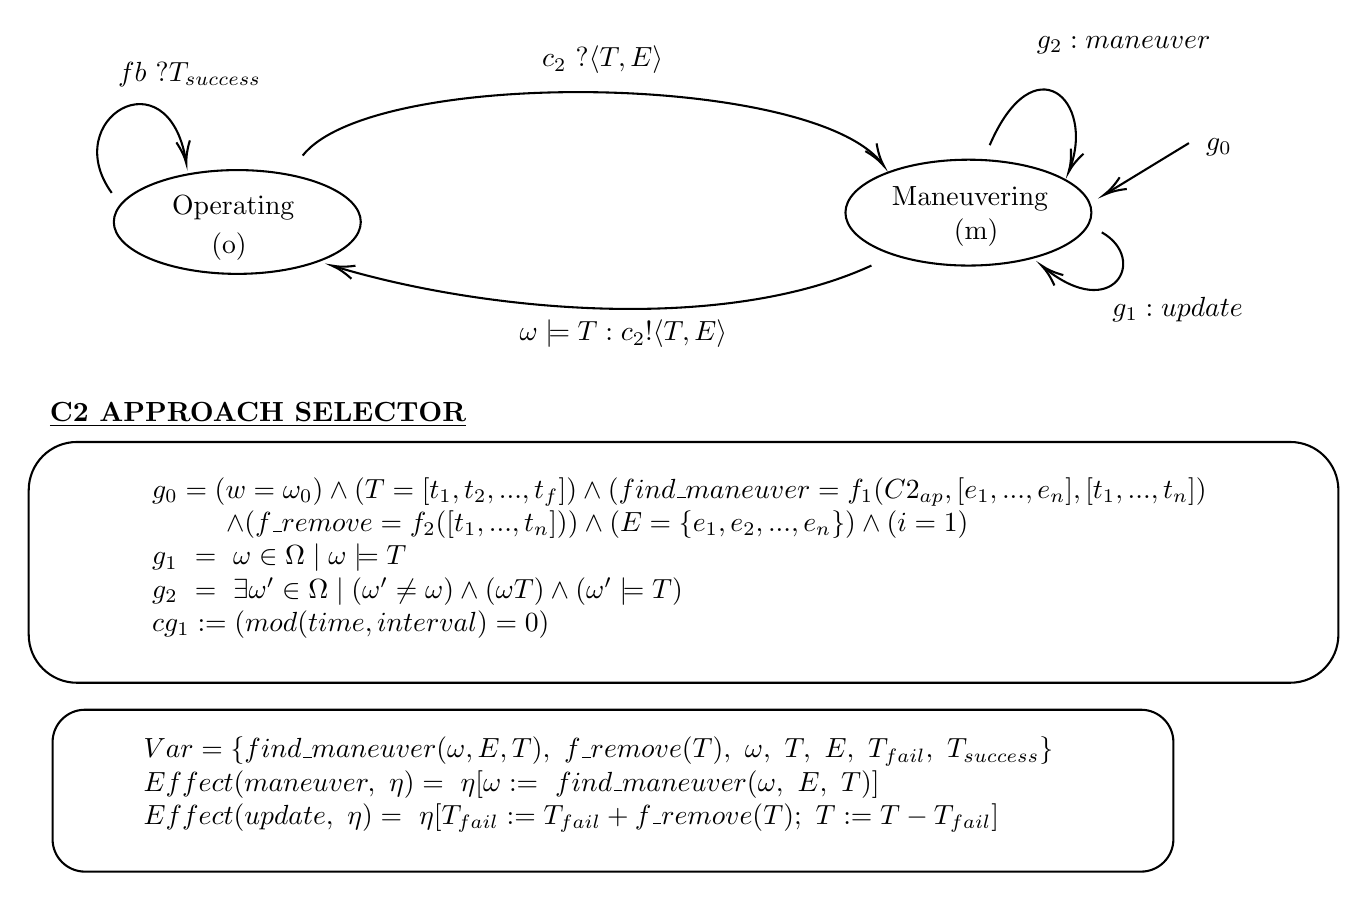
\begin{tikzpicture}[x=0.75pt,y=0.75pt,yscale=-1,xscale=1]
%uncomment if require: \path (0,420); %set diagram left start at 0, and has height of 420

%Curve Lines [id:da9480858267519683] 
\draw    (135.5,66) .. controls (169.16,23.43) and (380.22,25.94) .. (414.52,69.66) ;
\draw [shift={(415.5,71)}, rotate = 235.44] [color={rgb, 255:red, 0; green, 0; blue, 0 }  ][line width=0.75]    (10.93,-3.29) .. controls (6.95,-1.4) and (3.31,-0.3) .. (0,0) .. controls (3.31,0.3) and (6.95,1.4) .. (10.93,3.29)   ;
%Shape: Ellipse [id:dp6594609066072359] 
\draw   (44.5,98) .. controls (44.5,84.19) and (71.14,73) .. (104,73) .. controls (136.86,73) and (163.5,84.19) .. (163.5,98) .. controls (163.5,111.81) and (136.86,123) .. (104,123) .. controls (71.14,123) and (44.5,111.81) .. (44.5,98) -- cycle ;
%Shape: Ellipse [id:dp873836537729809] 
\draw   (397,93.5) .. controls (397,79.42) and (423.53,68) .. (456.25,68) .. controls (488.97,68) and (515.5,79.42) .. (515.5,93.5) .. controls (515.5,107.58) and (488.97,119) .. (456.25,119) .. controls (423.53,119) and (397,107.58) .. (397,93.5) -- cycle ;
%Curve Lines [id:da21020703050779688] 
\draw    (466.5,61) .. controls (487.68,11.75) and (517.59,39.15) .. (505.1,72.47) ;
\draw [shift={(504.5,74)}, rotate = 292.38] [color={rgb, 255:red, 0; green, 0; blue, 0 }  ][line width=0.75]    (10.93,-3.29) .. controls (6.95,-1.4) and (3.31,-0.3) .. (0,0) .. controls (3.31,0.3) and (6.95,1.4) .. (10.93,3.29)   ;
%Curve Lines [id:da14662580418826565] 
\draw    (520.5,103) .. controls (543.16,115.81) and (526.03,147.04) .. (493.02,120.26) ;
\draw [shift={(491.5,119)}, rotate = 400.46000000000004] [color={rgb, 255:red, 0; green, 0; blue, 0 }  ][line width=0.75]    (10.93,-3.29) .. controls (6.95,-1.4) and (3.31,-0.3) .. (0,0) .. controls (3.31,0.3) and (6.95,1.4) .. (10.93,3.29)   ;
%Straight Lines [id:da37650774099478246] 
\draw    (562.5,60) -- (523.21,83.96) ;
\draw [shift={(521.5,85)}, rotate = 328.63] [color={rgb, 255:red, 0; green, 0; blue, 0 }  ][line width=0.75]    (10.93,-3.29) .. controls (6.95,-1.4) and (3.31,-0.3) .. (0,0) .. controls (3.31,0.3) and (6.95,1.4) .. (10.93,3.29)   ;
%Rounded Rect [id:dp20897962983691354] 
\draw   (3.5,227.2) .. controls (3.5,214.39) and (13.89,204) .. (26.7,204) -- (611.3,204) .. controls (624.11,204) and (634.5,214.39) .. (634.5,227.2) -- (634.5,296.8) .. controls (634.5,309.61) and (624.11,320) .. (611.3,320) -- (26.7,320) .. controls (13.89,320) and (3.5,309.61) .. (3.5,296.8) -- cycle ;
%Rounded Rect [id:dp6489541210438411] 
\draw   (15,348.6) .. controls (15,339.98) and (21.98,333) .. (30.6,333) -- (539.4,333) .. controls (548.02,333) and (555,339.98) .. (555,348.6) -- (555,395.4) .. controls (555,404.02) and (548.02,411) .. (539.4,411) -- (30.6,411) .. controls (21.98,411) and (15,404.02) .. (15,395.4) -- cycle ;
%Curve Lines [id:da07722007259294938] 
\draw    (43.5,84) .. controls (17.76,48.36) and (70.43,16.64) .. (79.25,68.41) ;
\draw [shift={(79.5,70)}, rotate = 261.57] [color={rgb, 255:red, 0; green, 0; blue, 0 }  ][line width=0.75]    (10.93,-3.29) .. controls (6.95,-1.4) and (3.31,-0.3) .. (0,0) .. controls (3.31,0.3) and (6.95,1.4) .. (10.93,3.29)   ;
%Curve Lines [id:da13961356622291943] 
\draw    (409.5,119) .. controls (335.87,152.83) and (218.68,140.13) .. (150.52,119.31) ;
\draw [shift={(149.5,119)}, rotate = 377.15999999999997] [color={rgb, 255:red, 0; green, 0; blue, 0 }  ][line width=0.75]    (10.93,-3.29) .. controls (6.95,-1.4) and (3.31,-0.3) .. (0,0) .. controls (3.31,0.3) and (6.95,1.4) .. (10.93,3.29)   ;

% Text Node
\draw (102,91) node   [align=left] {Operating};
% Text Node
\draw (457,87) node   [align=left] {Maneuvering};
% Text Node
\draw (280,20) node    {$c_{2} \ ?\langle T,E\rangle $};
% Text Node
\draw (577,62) node    {$g_{0}$};
% Text Node
\draw (557,140) node    {$g_{1} :update$};
% Text Node
\draw (531,13) node    {$g_{2} :maneuver$};
% Text Node
\draw (317,260) node    {$ \begin{array}{l}
g_{0} =( w=\omega _{0}) \land ( T=[ t_{1} ,t_{2} ,...,t_{f}]) \land ( find\_maneuver=f_{1}( C2_{ap} ,[ e_{1} ,...,e_{n}] ,[ t_{1} ,...,t_{n}])\\
\ \ \ \ \ \ \ \ \land ( f\_remove=f_{2}([ t_{1} ,...,t_{n}])) \land ( E=\{e_{1} ,e_{2} ,...,e_{n}\}) \land ( i=1)\\
g_{1} \ =\ \nexists \omega \in \Omega \mid \omega \models T\\
g_{2} \ =\ \exists \omega '\in \Omega \mid ( \omega '\neq \omega ) \land ( \omega \nvDash T) \land ( \omega '\models T)\\
cg_{1} :=( mod( time,interval) =0)
\end{array}$};
% Text Node
\draw (460,103) node   [align=left] {(m)};
% Text Node
\draw (100,110) node   [align=left] {(o)};
% Text Node
\draw (278,369) node    {$ \begin{array}{l}
Var=\{find\_maneuver( \omega ,E,T) ,\ f\_remove( T) ,\ \omega ,\ T,\ E,\ T_{fail} ,\ T_{success}\}\\
Effect( maneuver,\ \eta ) =\ \eta [ \omega :=\ find\_maneuver( \omega ,\ E,\ T)]\\
Effect( update,\ \eta ) =\ \eta [ T_{fail} :=T_{fail} +f\_remove( T) ;\ T:=T-T_{fail}]
\end{array}$};
% Text Node
\draw (81,27) node    {$fb\ ?T_{success}$};
% Text Node
\draw (114,191) node   [align=left] {\textbf{\underline{C2 APPROACH SELECTOR}}};
% Text Node
\draw (290,152) node    {$\omega \models T:c_{2} !\langle T,E\rangle $};


\end{tikzpicture}